
\resetcounters

\bibliographystyle{asp2010}

\markboth{Berthoud}{HAWC Quicklook and Data Reduction}

\title{Online Data Reduction and Quicklook Tool for HAWC}
\author{Marc~G.~Berthoud
\affil{Yerkes Observatory, University of Chicago}}

\aindex{Berthoud, M.}

\begin{abstract}
The High-resolution Airborne Wide-band Camera (HAWC) is the facility
far-infrared imager for SOFIA, the Stratospheric Observatory For
Infrared Astronomy.  For best science return during SOFIA flights,
rapid inspection of reduced data is crucial. To optimize this process,
we have developed a web-based data viewing and analysis tool that
allows astronomers to rapidly access reduced files.  This web viewer
works in conjunction with the automatic data reduction pipeline: As
soon as the instrument closes a raw data file, the automatic pipeline
reduces the file and the reduced FITS files are copied to the on-board
web server. Linked to the experimenter's network, scientists and
engineers can call up the web viewer on their browser to analyze all
data products from the current flight's observations.  The web viewer
pages are generated by a Python script, with client-side operations in
Javascript. The software architecture is highly modular, so various
parts can be reconfigured or used in other projects.  The HAWC
automatic pipeline and the web viewer were used during our last
instrument tests in the spring of 2012. These tools significantly
improved the efficiency of lab operations. We expect similar gains
when using HAWC during flight operations on SOFIA. An online demo of
the HAWC web viewer is available at
\url{http://bussard.yerkes.uchicago.edu/hawcdemo}.\end{abstract}

\section{Introduction}

The Stratospheric Observatory For Infrared Astronomy (SOFIA) is NASA's
new airborne observatory. The telescope has a 2.7m diameter mirror
mounted in a modified Boeing 747 aircraft. First light with SOFIA was
achieved in May 2010 \citep{herter12}. The High-resolution Airborne
Wide-band Camera (HAWC) will be the facility far-infrared camera for
SOFIA.

HAWC currently uses a single bolometer array in a $32\times12$
rectangular format. Before flying, it will be upgraded with dual
$64\times40$ arrays and polarimetric capabilities. Filters in the
six-position filter wheel cover the spectral range from 50 to $250\mu
m$. Lenses in each filter position allow diffraction-limited imaging in
each band. Normal imaging uses the SOFIA secondary mirror assembly
(SMA), chopping in a two-position mode.

There are special challenges when observing on SOFIA. To ensure high
quality observations during the flight, a preliminary data reduction
is needed on a time scale of a few minutes. After the flight, the
SOFIA Data Cycle System (DCS) \citep[see][]{P050_adassxxii} manages
post-flight data reduction and archival storage. To satisfy these
requirements, the HAWC Data Reduction Pipeline (DRP) needs the
flexibility to operate in these different modes. We decided to use the
same basic pipeline package in both environments, with a web-based data
viewer as the main in-flight data analysis tool.

\section{HAWC Data Reduction Pipeline and Web Viewer}

The overall design goal was to divide the software into simple,
self-contained modules with limited dependencies and interfaces. This
keeps the code flexible to facilitate changes and allows parts of the
software to be re-used for other projects. Most of the code is written
in Python, using the popular numpy, pyfits\ooindex{PyFITS, ascl:1207.009} and configobj
libraries. All parts of the software write log files upon execution
and can be customized using configuration files.

\begin{figure}
\plotone{part7/Berthoud_P006/P006_f1.eps}

\caption{HAWC in-flight data reduction software architecture: The data
  flows from left to right. The IRC software controls the instrument
  and records the data. The data is then reduced on the DRP computer,
  which also hosts the web server that provides data to clients on the
  Experimenter Network.}

\label{fig_struct}

\end{figure}

The overall structure of the HAWC data reduction software is shown in
Figure \ref{fig_struct}. The HAWC data is reduced on a central server
such that scientists access the reduced data products without needing
to reduce the data on their own computers. This configuration is
different from many other instruments where the data reduction is done
on stand-alone computers. For HAWC custom data reduction, it is still
possible to reduce data on stand-alone computers. A rudimentary data
reduction GUI has been developed for that case.

\subsection{Data Reduction Pipeline Core Package}

The Data Reduction Pipeline (DRP) core package performs all HAWC data
reduction. HAWC has two science instrument modes, chop-nod and
chop-scan, as well as several diagnostic modes. In the configuration
file, the DRP core can be adapted for different data reduction
requirements, including the sequencing of pipe steps.

\begin{figure}[!ht]
\begin{minipage}{\textwidth}
\leavevmode \centering
\raisebox{-0.5\height}{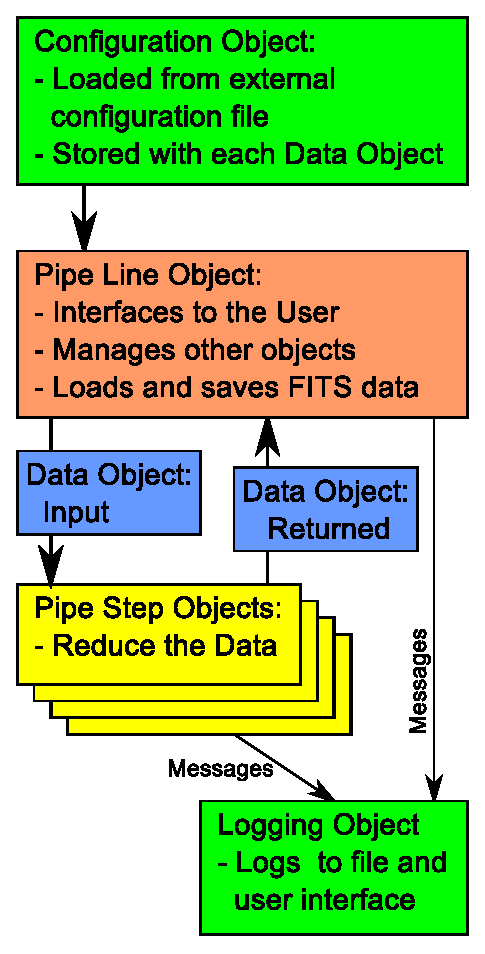
\includegraphics[width=0.3\textwidth]{part7/Berthoud_P006/P006_f2a.eps}}
\hfil
\hfil
\raisebox{-0.5\height}{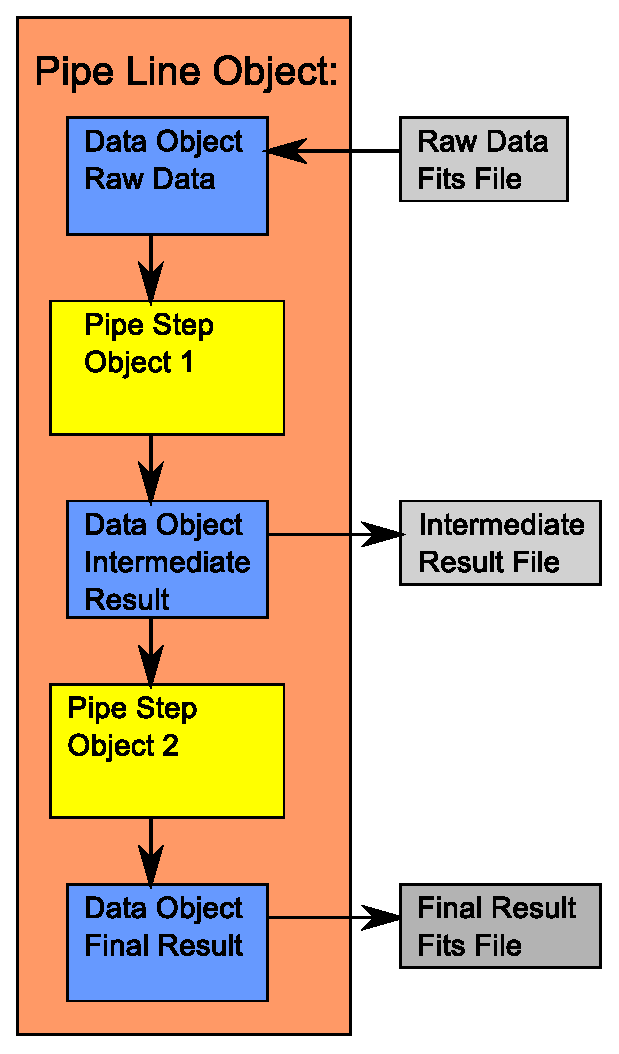
\includegraphics[width=0.3\textwidth]{part7/Berthoud_P006/P006_f2b.eps}}
\hfil
\raisebox{-0.5\height}{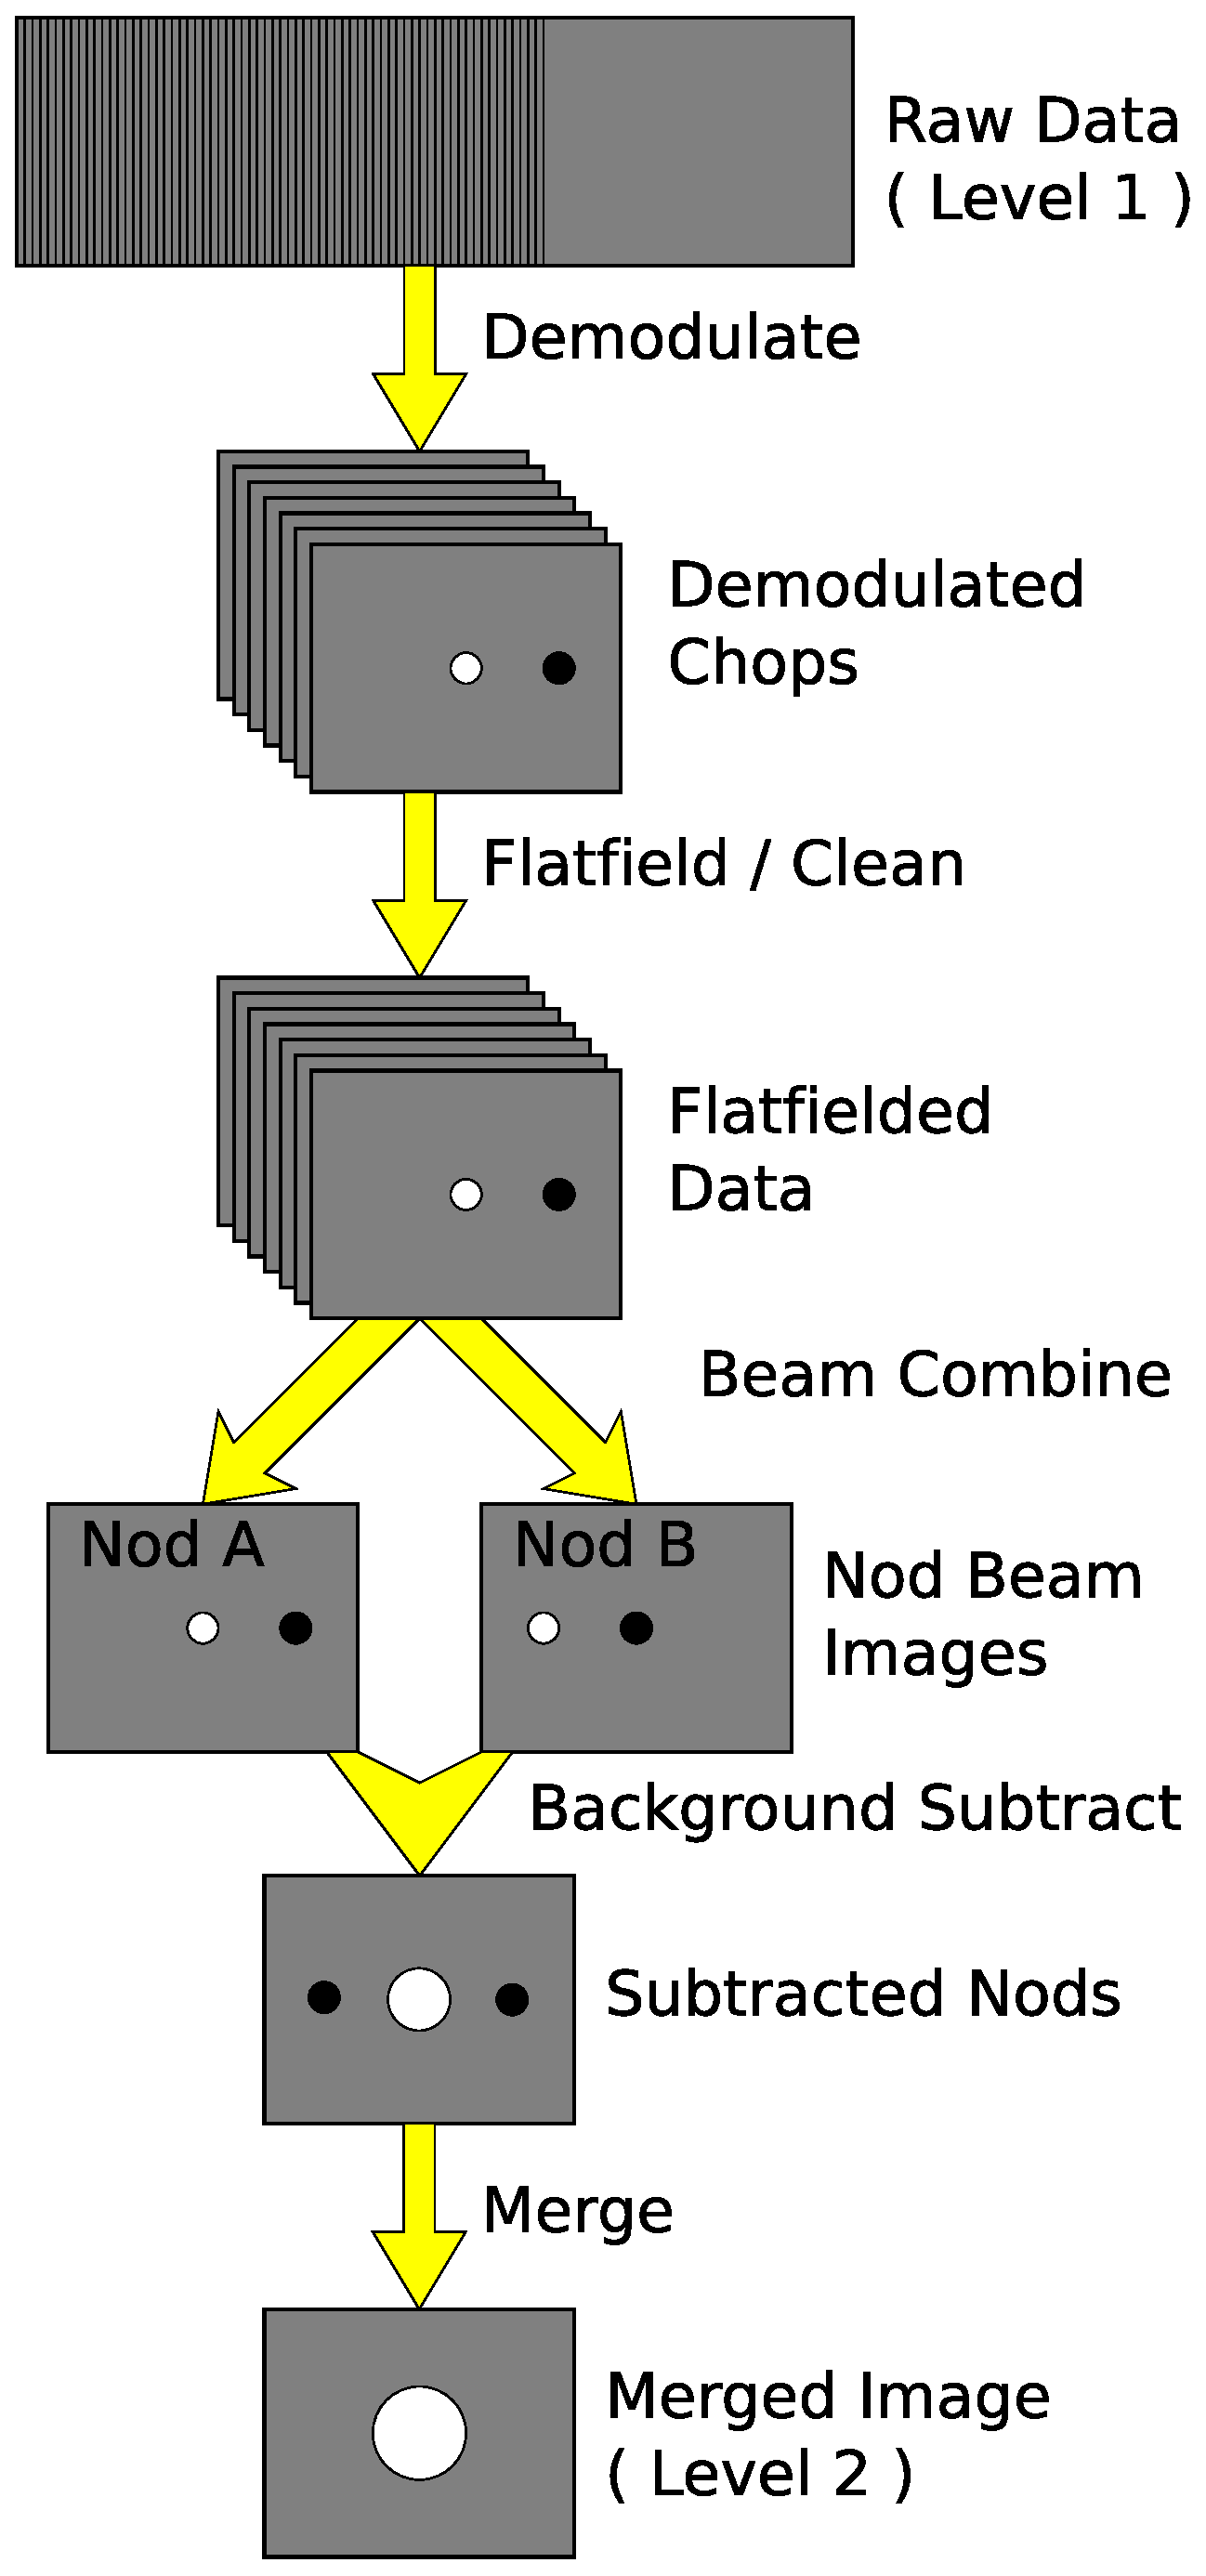
\includegraphics[width=0.3\textwidth]{part7/Berthoud_P006/P006_f2c.eps}}
\end{minipage}

\caption{Architecture and processing sequence of the DRP core: The
  diagram on the left shows the object structure of the software: The
  overall process is managed by the Pipe Line object. This object
  creates and calls Pipe Step objects, each responsible for a data
  reduction step. Data is stored and exchanged in Data objects, each
  containing the equivalent of a FITS file, including headers and
  multiple HDUs. A common configuration object is accessed by all
  objects, which also send messages to common loggers. The diagram in
  the center illustrates the flow of data through a two-step
  pipeline. The diagram on the right gives an example of the five
  necessary pipe steps to reduce chop-nod data.}

\label{fig_core}
\end{figure}

The HAWC DRP core package is
based on the FORCAST pipeline developed by Luke Keller, Alfred Lee
and the author.
The architecture and processing sequence are
illustrated in Figure \ref{fig_core}. Each pipe step receives a data
object and returns one to the pipeline. Individual pipe steps store
intermediate results for reducing multiple files of a single
astronomical observation. For example, the merge step in Figure
\ref{fig_core} combines the data from all input files. The steps can
also call code in other languages such as C or IDL.

\subsection{In-flight Data Reduction and Analysis}

As shown in Figure \ref{fig_struct}, raw HAWC data is recorded by the
HAWC IRC. This software is a version of the IRC software framework
customized for HAWC. The IRC was developed at Goddard Space Flight
Center and has been used for several other instruments
\citep[see][]{staguhn06}. The HAWC automatic pipeline detects and
sends new raw files through a Pipe Line object, which is configured
to store all intermediate and final data products as FITS files.

\begin{figure}[!ht]
\plotone{part7/Berthoud_P006/P006_f3.eps}

\caption{Screenshots of the HAWC web viewer: The shot on the left
  shows the data window. The user selects observation, file, and pipe
  step in the upper left. The center contains image information, while
  the image display and analysis tools are on the upper right. The
  image display is below. The three screenshots on the right show the
  observation list at the top, the DRP log in the middle, and a data
  plot at the bottom. The Web Viewer can also display FITS tables and
  header information.}

\label{fig_screen}

\end{figure}

The HAWC web viewer provides access to these FITS files. This simple
flat file data storage makes it easy to add or update files. The user
interface for the web viewer is shown in Figure \ref{fig_screen}. The
web viewer is a Python WSGI script run by an Apache server. The image
viewer on the client is an independent Javascript package which
handles data analysis by the user. Image data, as well as log and file list
updates, are transferred via AJAX. Optional access control is
established by htaccess on the web server.

\section{Current Status - Outlook}

The pipeline and the web viewer were used during our 2012 laboratory
tests. The quick automatic data reduction increased testing efficiency
and made the results easily available to remote collaborators.
The web viewer was also used to share preliminary results during recent
observations at the Caltech Submilimeter Observatory.

HAWC is currently scheduled to be commissioned in 2015 with various
upgrades, including rotating half-wave plates and two $64\times40$
pixel arrays that simultaneously observe the two components of
linearly polarized light. We will adapt the data reduction and
analysis tools for the requirements of polarized observations.

\acknowledgements This work has been supported by NASA though the
SOFIA observatory. Special thanks to the HAWC team for ideas and support.

\bibliography{editor}
